%%==========================================================================%%
%% Author : Sa�udo Olmedo, Ignacio                                          %%
%% Author : S�nchez Barreiro, Pablo                                         %%
%% Version: 1.2, 23/04/2014                                                 %%
%%                                                                          %%
%% Memoria del Proyecto Fin de Carrera                                      %%
%% M2M/MetamodeloCassandra                                                  %%
%%==========================================================================%%
AMPLIAR Y CORREGIR GRAMATICALMENTE
Previo paso a la definici�n de las reglas de transformaci�n entre modelos necesitamos definir un meta-modelo de origen y un meta-modelo de destino.Como hab�amos descrito en el capitulo anterior la base del proceso de transformaci�n entre modelos parte del meta-modelo. El meta-modelo utilizado como origen de UML en este proyecto es el que nos proporciona Epsilon, dicho meta-modelo sigue el est�ndar de UML 2.0. A parte del meta-modelo de UML nos hace falta un meta-modelo que defina el lenguaje de Cassandra. Dicho meta-modelo fue proporcionado por Pablo S�nchez Barreiro. Este meta-modelo se construyo por medio de la abstracci�n de las caracter�sticas de Cassandra. El meta-modelo sufri� algunos cambios respecto al inicial debido a exigencias del proyecto. La Figura~\ref{back:fig:metamodeloCassandra} muestra un diagrama de clase UML que representa el modelo de datos. Este tipo de modelo es el origen del proceso de transformaciones entre modelos que queremos crear.

\begin{figure}[!tb]
  \centering
  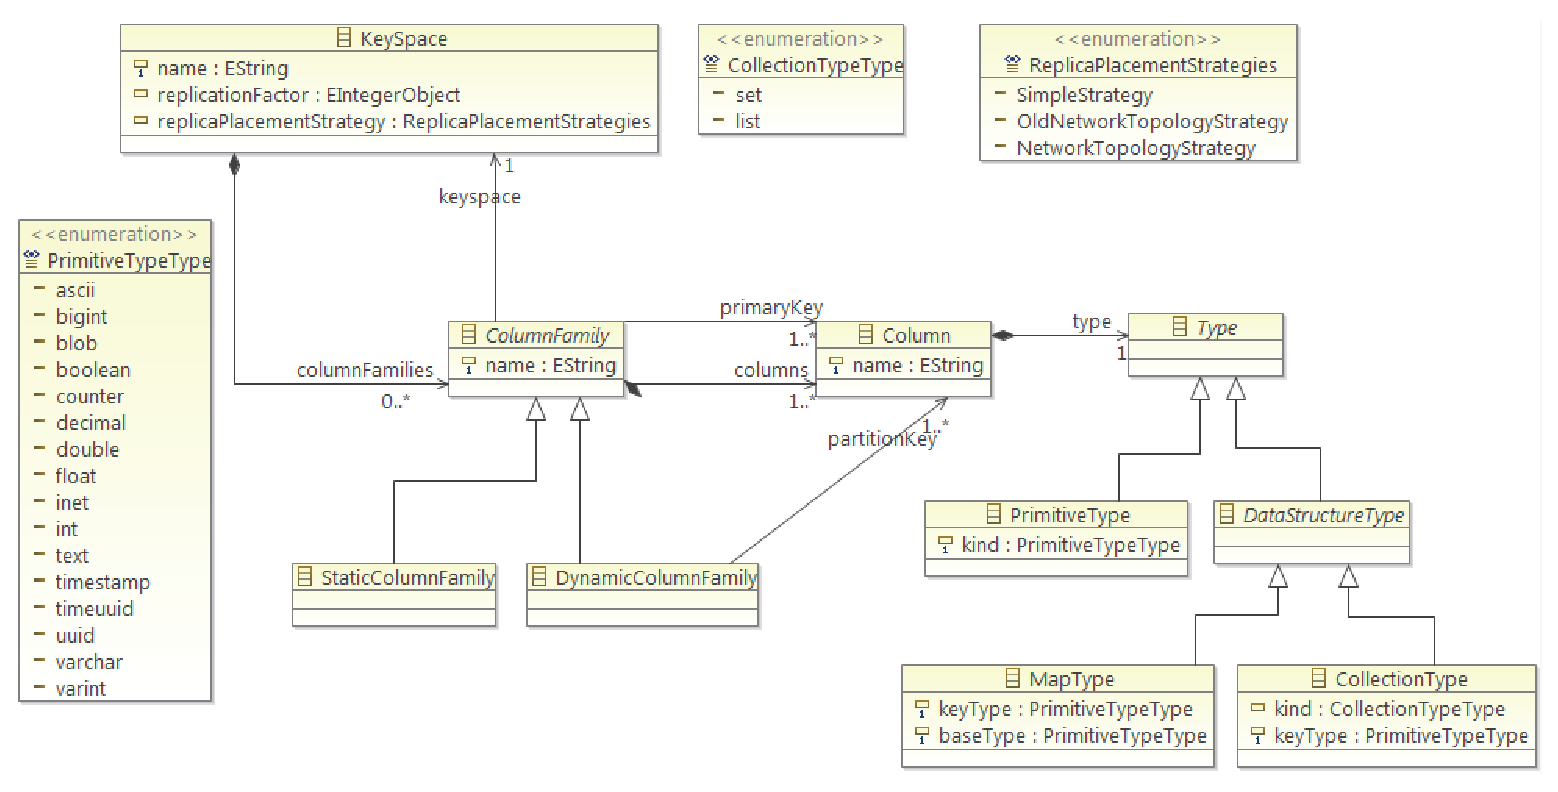
\includegraphics[width=.8\linewidth]{m2m/images/ecoreDiag.eps} \\
  \caption{Metamodelo Cassandra}
  \label{back:fig:metamodeloCassandra}
\end{figure}

A continuaci�n se detallan los aspectos mas importantes del meta-modelo de Cassandra.

De acuerdo con el modelo de Cassandra, el elemento ra�z de cualquier esquema orientado a columnas es el Key Space, el Key Space es el equivalente a la base de datos en el modelo relacional, la meta-clase Key Space cuenta con los atributos: nombre utilizado para denominar el Key Space, [cassandra] replicationFactor que representa el n�mero de servidores de Cassandra de los que se debe guardar un registro u obtener una respuesta al recuperar alg�n registro y replicaPlacementStrategy que es la estrategia de replicaci�n que se va a tomar, estrategias tenemos tres tipos: %[http://www.datastax.com/docs/1.0/cluster_architecture/replication]:

\begin{enumerate}
\item SimpleStrategy: Esta estrategia es la estrategia de replicaci�n utilizada por defecto al crear un KeySpace utilizando Cassandra. Es utilizada para cl�steres de data centers simples.
\item NetworkTopologyStrategy: Utilizada cuando se tiene (o se va a tener) el cl�ster desplegado a trav�s de m�ltiples data centers. Esta estrategia especifica cu�ntas r�plicas se desean en cada data center.
\item OldNetworkTopologyStrategy: Se utiliza para proporcionar retro compatibilidad con instalaciones Cassandra antiguas.
\end{enumerate}

A continuaci�n tenemos la meta-clase ColumnFamily (CF) equivalente a las tablas en el modelo relacional, dentro de las CF encontramos dos tipos: las StaticColumnFamily y las DynamicColumnFamily. Recordamos que las Static Column Family son el equivalente a las tablas en el modelo relacional, sin embargo las Dynamic Column Family son utilizadas para la recuperaci�n de datos eficiente, algo similar a las vistas del modelo relacional. %[http://www.datastax.com/docs/1.1/ddl/column_family#dynamic-column-families].

A la hora de definir las claves de las Column Family hay que tener en cuenta el orden, en CQL el orden de definici�n de las claves importa, en la primera columna se define la Partition Key esta tiene la propiedad de que todas las filas que comparten la misma Partition Key se almacenan en el mismo nodo f�sico %[http://www.datastax.com/docs/1.1/ddl/indexes].
Adem�s, la inserci�n, actualizaci�n o eliminaci�n de filas que comparten la Partition Key para una CF determinada se realizan de forma at�mica. Es posible tener una Partition Key compuesta, es decir, una Partition Key formada por varias columnas, en CQL esto se define utilizando par�ntesis para delimitar el conjunto de partici�n.

Dentro de las Column Family encontramos Columns estos son los valores que se almacenan en las Column Families, estas Columns tienen como atributos un nombre y un tipo de dato. 
Dentro de los tipos de dato que puede ser una columna encontramos dos tipos, PrimitiveType y DataStructureType, el primero define los tipos primitivos, por ejemplo entero, texto, uuid, etc..
DataStructureType define las colecciones, estas pueden ser de dos tipos MapType o bien CollectionType, ambas  tiene un atributo llamado KeyType para definir el tipo primitivo que las caracteriza. MapType cuenta con un atributo llamado baseType de tipo primitivo que define el segundo tipo de dato del mapa. Dentro de CollectionType encontramos un atributo llamado kind que define el tipo de colecci�n que vamos a utilizar esta puede ser o bien tipo set o tipo list. M�s adelante se explica que caracter�sticas re�ne cada colecci�n y mapa y cuando se utilizan.
